\chapter{Functional Renormalization and Quantum Gravity}\label{chap:EHT}
After the formal introduction of the physical and mathematical concepts in the last chapters, we are now able to motivate and formulate the key idea of the Asymptotic Safety approach to quantum gravity, which aims at finding a quantum field theoretical description of gravity within the language of the Functional Renormalization Group. This chapter briefly discusses the requirements for the existence of such a theory. We proceed by solving the flow equation for quantum gravity within the Einstein-Hilbert truncation in a transverse-traceless spin-two graviton approximation and investigate its fixed point structure. 
\vspace{-0.6cm}
\section{Asymptotic Safety}
Asymptotic Safety generalizes the concept of Asymptotic Freedom known as a property of certain gauge theories. The latter one is based on the idea, that the interaction of particles becomes asymptotically weak in the high-energy limit. In the language of the FRG this means, that the UV behavior of such theories is governed by a non-interacting, Gaussian fixed point,  allowing perturbative calculations. Maybe the most popular example for an asymptotically free theory is Quantum  Chromodynamics (QCD), the theory of the strong interaction. In 1978,  Steven Weinberg proposed the Asymptotic Safety scenario for gravity, based on the existence of an interacting, Non-Gaussian fixed point, rendering the theory non-perturbatively renormalizable in the UV \cite{Weinberg1980}. The main advantage compared to other approaches is, that there is no need to introduce new symmetries, extra dimensions or other additional complications. The key requirements for an asymptotically safe quantum field theory of gravity can be summarized as follows: 
\begin{enumerate}
	\item The existence of an UV-attractive NGFP of the Renormalization Group flow of $\Gammak$ has to be guaranteed. 
	\item For the predictivity of the theory, it is crucial to be able to fix the trajectory $\Gammak$ by a finite amount of measurements, i.\,e. the corresponding UV hypersurface $\Sigma_{\mathrm{UV}}$ of the NGFP should be of finite dimension: 
	\begin{equation*}
		\operatorname{dim}\Sigma_{\mathrm{UV}} < \infty.
	\end{equation*} 
\end{enumerate} 
We want to probe these requirements in the following by computing the running of the Newton constant $G_k$ and the cosmological constant $\Lambda_k$ in a pure-gravity setting. \\
For a more detailed discussion of current Asymptotic Safety research, we refer the interested reader to \cite{Eichhorn2018}. Recently, very detailed textbooks covering both, the physical and the mathematical concepts of Asymptotic Safety, have been released. For a complete treatment of the subject it is worth to have a look at \cite{Percacci2017} or \cite{ReuterSaueressig_2019}.
\vspace{-0.6cm}
\section{Einstein-Hilbert Truncation}
Solving the flow equation analytically is nothing but impossible. Therefore it is unavoidable to truncate the initially infinite dimensional theory space to a finite subspace, to be able to find approximated solutions. It is important, that all terms, that are invariant under the imposed symmetry, i.\,e. invariant under diffeomorphism transformations, need to be taken into account. The easiest truncation fulfilling this requirement is the \textit{Einstein-Hilbert truncation}. In 1996, Martin Reuter was the first to successfully investigate quantum gravity within the Einstein-Hilbert truncation \cite{Reuter1996}. He was able to prove the existence of a NGFP for a pure-gravity setting. This truncation takes only the scalar curvature $\Ricci$ and the cosmological constant $\Lambda$ into account and therefore the truncated subspace is $2$-dimensional\footnote{Recently, more sophisticated truncations including higher-order curvature terms ($\Ricci^2$, $f(\Ricci)$, $R^{\mu\nu}R_{\mu\nu}$ \dots) have been investigated, see e.\,g. \cite{AlkoferSaueressig2018}.}.\\ The full Einstein-Hilbert  truncation reads:
\begin{align}
	\Gammak = 2\kappa^2Z_{h,k} \int_x \sqrt{g} \ [-\mathcal{R} + 2\Lambda_k] + \mathcal{S}_{\text{gf}} + \mathcal{S}_{\text{gh}},
\label{eqn:EHtruncation}
\end{align}
where we abbreviated $\kappa^2 = \left(32\pi G\right)^{-1}$. Since we don't need to consider the gauge fixing action $\mathcal{S}_{\text{gf}}$ and the Non-Abelian ghost action $\mathcal{S}_{\text{gh}}$ for the calculation performed in this chapter, we won't specify their explicit forms at this point. We will come back to this discussion at the beginning of chapter \ref{chap:Matter}.\\
 The index $k$ indicates the \textit{running} i.\,e. the scale dependence of the cosmological constant and the wave function renormalization $Z_{h,k}$. It is quite convenient to define the running Newton coupling as 
 \begin{equation}
 	G_k = G \cdot \left(Z_{h,k}\right)^{-1}.
 \end{equation}
Up to this point, we did not care about the dimensionality of the two couplings. As already mentioned, one usually works with dimensionless couplings when solving the flow equation. \\
We therefore define the dimensionless renormalized cosmological constant 
\begin{align}
	\lambda_k = \Lambdak\cdot k^{-2}
\end{align}
and Newton constant
\begin{align}
	g_k = G_k\cdot k^{d-2} \ \overset{(d=4)}{=} \ G_k\cdot k^{2}.
\end{align}
After these redefinitions, we can already compute the l.\,h.\,s. of the flow equation, i.\,e. the scale derivative w.\,r.\,t. the RG time $t$. The derivative only acts on $\lambda_k$ and $g_k$.
\begin{align}
	\partial_{t}\Gamma_{k} = 2\kappa^2 Z_{k,h}\int_x \sqrt{g} \left\{\eta_h\mathcal{R}+2\left(k^2(\partial_t\lambda_k) + \Lambda_k(2 - \eta_h)\right)\right\}.
	\label{eqn:LHS}
\end{align}
Here we introduced the \textit{anomalous dimension} $\eta_h$, defined as
\begin{align}
	\eta_h=-\partial_t \ln Z_{h,k} = -\frac{\partial_tZ_{h,k}}{Z_{h,k}}.
\end{align} 
We find terms of order $\sim\sqrt{g}$ and order $\sim\sqrt{g}\Ricci$. The r.\,h.\,s. of the flow equation is assumed to admit an expansion in terms of invariants, which will also be of order $\sim\sqrt{g}$ and $\sim\sqrt{g}\mathcal{R}$ since we are working in the Einstein-Hilbert truncation\footnote{There will also appear terms of higher order in curvature, but we will drop them.}. This will allow us to determine the $\beta$-function for $\lambda_k$ and the explicit form of $\eta_h$ by a comparison of the terms of these orders on both sides of the flow equation.
The $\beta$-function for $g_k$ follows directly from the anomalous dimension:
\begin{align}
	\beta_g = \partial_t g_k = \left(2 + \eta_h\right)g_k.
	\label{eqn:beta_gk}
\end{align}
At this point, we want to use the idea of the background field approximation. We assume a linear split of the metric into a background field $\bar{g}$ and a fluctuation field $h$, as described in  equation (\ref{eqn:metric_split}). The approximation at this point is, that in the following, we set all fluctuations to zero, i.\,e. we evaluate all derivatives etc. at $g=\bar{g}$. We will critically review this approximation in chapter \ref{chap:BGindependence}. In general, there is no conceptual need to fix the background metric, it nevertheless is really useful to choose specific classes of backgrounds for certain computations, since this can simplify calculations a lot. We exploit the freedom of choosing a spherical background. On the four-sphere $\mathbb{S}^4$, which is a maximally symmetric space\footnote{Maximally symmetric spaces are characterized by the fact, that they have the same number of symmetries as ordinary Euclidean space.}, the Riemann tensor and the Ricci tensor can be written as multiples of the curvature scalar:
\begin{equation}
\begin{aligned}
	\bar{R}_{\mu\nu} &= \frac{1}{4} \ \bar{g}_{\mu\nu} \bar{\mathcal{R}}\\[10pt]
	\bar{R}_{\mu\nu\rho\sigma} &= \frac{1}{12} \ (\bar{g}_{\mu\rho}\bar{g}_{\nu\sigma} - \bar{g}_{\mu\sigma}\bar{g}_{\nu\rho}) \bar{\mathcal{R}}.
\end{aligned}	
\end{equation}
The bar in this notation refers to the background $\bar{g}$. The inversion of the two-point function on general curved backgrounds is non-trivial. We need to find a suitable tensor basis for the decomposition of the metric fluctuation $h_{\mu\nu}$. We choose a \textit{York decomposition} and find:
\begin{equation}
	h_{\mu v}=h_{\mu v}^{\mathrm{TT}}+\bar{\nabla}_{\mu} \xi_{v}+\bar{\nabla}_{v} \xi_{\mu}+\left(\bar{\nabla}_{\mu} \bar{\nabla}_{v}-\frac{1}{d} \bar{g}_{\mu v} \bar{\Delta}\right) \sigma+\frac{1}{d} \bar{g}_{\mu v} h.
	\label{eqn:York}
\end{equation}
Here, $ h_{\mu\nu}^{\text{TT}}$ is a transverse-traceless, spin-two degree of freedom, $\xi_{\mu}$ is transverse and carries a spin-one d.\,o.\,f. and $\sigma$ and $h$ have spin zero. For a more detailed motivation of the York decomposition, we refer to appendix \ref{chap:AppA}.\\
As a further approximation, we only take the contribution from the spin-two graviton mode $h_{\mu\nu}^{\text{TT}}$ into account\footnote{This choice is motivated by the fact, that the spin-two mode carries the most degrees of freedom. From the $10$ initial d.\,o.\,f. in this decomposition, $4$ can be removed via gauge fixing, the remaining $6$ are divided into $5$ from the $h_{\mu\nu}^{\text{TT}}$ mode and $1$ for the trace mode $h$.}. The other modes are included later on in chapter \ref{chap:Matter}, when we couple matter to the system. \\
Our starting point for the computation of the r.\,h.\,s. of the flow equation is the transverse-traceless graviton two-point function:
\begin{align}
\Gamma_{k, h^{\text{TT}}h^{\text{TT}}}^{(2)} = \frac{Z_k}{32\pi}\left(\bar{\Delta} - 2\Lambda_k+\frac{2}{3}\bar{\mathcal{R}}\right).
\end{align}
Here, we used the definition of the Laplace operator, given by $\Delta = -\nabla^2$. We use a regulator of the form 
\begin{align}
R_k  = \eval{\Gamma_{h^{\text{TT}}h^{\text{TT}}}^{(2)}}_{\Lambda_k=\bar{\mathcal{R}}=0} \cdot r_k\left(\frac{\bar{\Delta}}{k^2}\right),
\end{align}
with a Litim-type shape function (\ref{eqn:Litim}). This allows us to determine the full propagator
\begin{equation}
	G_{k, h^{\text{TT}}h^{\text{TT}}} := \left(\Gamma_{k, h^{\text{TT}}h^{\text{TT}}}^{(2)} + R_k\right)^{-1} = \frac{32\pi}{Z_{h,k}}\left(\bar{\Delta}\left(1+r_k\right) -2\Lambda_k + \frac{2}{3}\bar{\mathcal{R}}\right)^{-1}
\end{equation}
and the scale derivative of the regulator
\begin{equation}
	\partial_t R_k =  \frac{Z_{h,k}}{32\pi}\bar{\Delta}\left(\partial_tr_k - \eta_hr_k\right).
\end{equation}
The computation of the r.\,h.\,s. of the flow equation is in general very hard because it involves the computation of a functional trace of a function depending on the Laplacian on a curved background. We can use \textit{heat-kernel techniques} to solve such equations. Heat-kernel computations are based on a curvature expansion in powers of the curvature scalar $\mathcal{R}$. For more details, have a look at the second part of appendix \ref{chap:AppA}.\\
The previously obtained results lead us to
\begin{equation}
\frac{1}{2}\operatorname{Tr}\left[G_{k, h^{\text{TT}}h^{\text{TT}}}\ \partial_t R_k\right] = \frac{1}{2}\operatorname{Tr}\left[\frac{\bar{\Delta}\left(\partial_t r_k - \eta_h r_k\right)}{\bar{\Delta}(1+r_k)-2\Lambda_k+\frac{2}{3}\bar{\mathcal{R}}}\right].
\end{equation}
We proceed by expanding this expression around vanishing curvature:
\begin{align}
\resizebox{.9 \textwidth}{!}{$
\frac{1}{2}\operatorname{Tr}\left[G_{k, h^{\text{TT}}h^{\text{TT}}}\ \partial_t R_k\right] = \frac{1}{2}\operatorname{Tr}\left[\frac{\bar{\Delta}\left(\partial_t r_k - \eta_h r_k\right)}{\bar{\Delta}(1+r_k)-2\Lambda_k}\right] - \frac{1}{3}\bar{\mathcal{R}}\operatorname{Tr}\left[\frac{\bar{\Delta}\left(\partial_t r_k - \eta_h r_k\right)}{\left(\bar{\Delta}(1+r_k)-2\Lambda_k\right)^2}\right] + \mathcal{O}(\mathcal{R}^2).$
}
\end{align}
We evaluate these two terms separately using the heat-kernel formulas presented in appendix \ref{chap:AppA}. The result for the first term reads
\begin{align}
\frac{1}{2}\operatorname{Tr}\left[\frac{\bar{\Delta}\left(\partial_t r_k - \eta_h r_k\right)}{\bar{\Delta}(1+r_k)-2\Lambda_k}\right] &= \frac{1}{2}\frac{1}{(4\pi)^2}\int_x \sqrt{\bar{g}} \left[5\Phi_2^1(-2\Lambda_k) - \frac{5}{6}\bar{\mathcal{R}}\Phi^1_1(-2\Lambda_k)\right] \\[10pt]
&= \frac{1}{2}\frac{1}{(4\pi)^2}\int_x \sqrt{\bar{g}}\left[\frac{1}{1-2\lambda_k}\left(5\left(1-\frac{\eta_h}{6}\right) - \frac{5}{3}\bar{\Ricci}\left(1-\frac{\eta_h}{4}\right)\right)\right],\nonumber
\label{eqn:hk41_test}
\end{align}
with the definition of threshold functions 
\begin{equation}
\begin{aligned}
	\Phi_n^p(\omega) &= \frac{1}{\Gamma(n)}\int_0^{\infty}\dd z \ z^{n-1} \frac{z(-2zr_k(z)-\eta_{\Psi}r_k(z))}{(z(1+r_k(z))+\omega)^p}\\[10pt] 
	&= \frac{1}{\Gamma(n)}\frac{1}{\left(1+\omega\right)^p}\left(\frac{2}{n} - \frac{\eta_{\Psi}}{n(n+1)}\right).
\end{aligned}
\label{eqn:threshold}
\end{equation}
In the last step, we evaluated the threshold functions for the Litim-type shape function. We used $\eta_\Psi$, since we want to keep this formula as general as possible and we will use it multiple times for different fields throughout this thesis. Analogously, the second term in our expansion reads
\begin{align}
	-\frac{1}{3}\bar{\mathcal{R}}\operatorname{Tr}\left[\frac{\bar{\Delta}\left(\partial_t r_k - \eta_h r_k\right)}{\left(\bar{\Delta}(1+r_k)-2\Lambda_k\right)^2}\right] &= -\frac{1}{2}\frac{1}{(4\pi)^2}\int_x \sqrt{\bar{g}} \ \frac{10}{3}\bar{\Ricci}\ \Phi_2^2(-2\Lambda_k)\\
	&=  -\frac{1}{2}\frac{1}{(4\pi)^2}\int_x \sqrt{\bar{g}}\left[\frac{1}{(1-2\lambda_k)^2}\left( \frac{10}{3}\bar{\Ricci}\left(1-\frac{\eta_h}{6}\right)\right)\right].\nonumber
	\label{eqn:hk42}
\end{align}
With these results, we are able to determine the $\beta$-function for the cosmological constant, simply by comparing the order $\sim\sqrt{\bar{g}}$ terms occurring on the l.\,h.\,s. of the flow equation and the results from the heat-kernel expansion of the functional trace:
\begin{align}
	\beta_{\lambda} = \partial_t\lambda_k = -4\lambda_k + \frac{\lambda_k}{g_k} \partial_t g_k + \frac{5}{4\pi}g_k\frac{1-\frac{\eta_h}{6}}{1-2\lambda_k}.
\end{align}
Additionally, we find an expression for the anomalous dimension $\eta_h$ by comparing the terms of order $\sim\sqrt{\bar{g}}\bar{\Ricci}$:
\begin{align}
\eta_h = -\frac{5g_k}{3\pi} \left(\frac{1-\frac{\eta_h}{4}}{1-2\lambda_k} + 2\frac{1-\frac{\eta_h}{6}}{(1-2\lambda_k)^2}\right).	
\end{align}
To find the fixed points for this truncated solution, we use \verb|Mathematica| to solve the equation
\begin{equation}
	\vec{\beta} = \begin{pmatrix}\beta_g\\ \beta_{\lambda}\end{pmatrix} \overset{!}{=}  \begin{pmatrix}0\\ 0\end{pmatrix}.
\end{equation}
We arrive at the following values for the Newton coupling and the cosmological constant at the NGFP:
\begin{align}
	(g_k^*, \lambda_k^*) = (0.86, 0.18).
\end{align}
The critical exponents of the fixed point are given by the complex conjugated pair
\begin{align}
	\theta_{1,2} = 2.9 \pm 2.6i. 
\end{align}
\begin{figure}[t]
\centering
	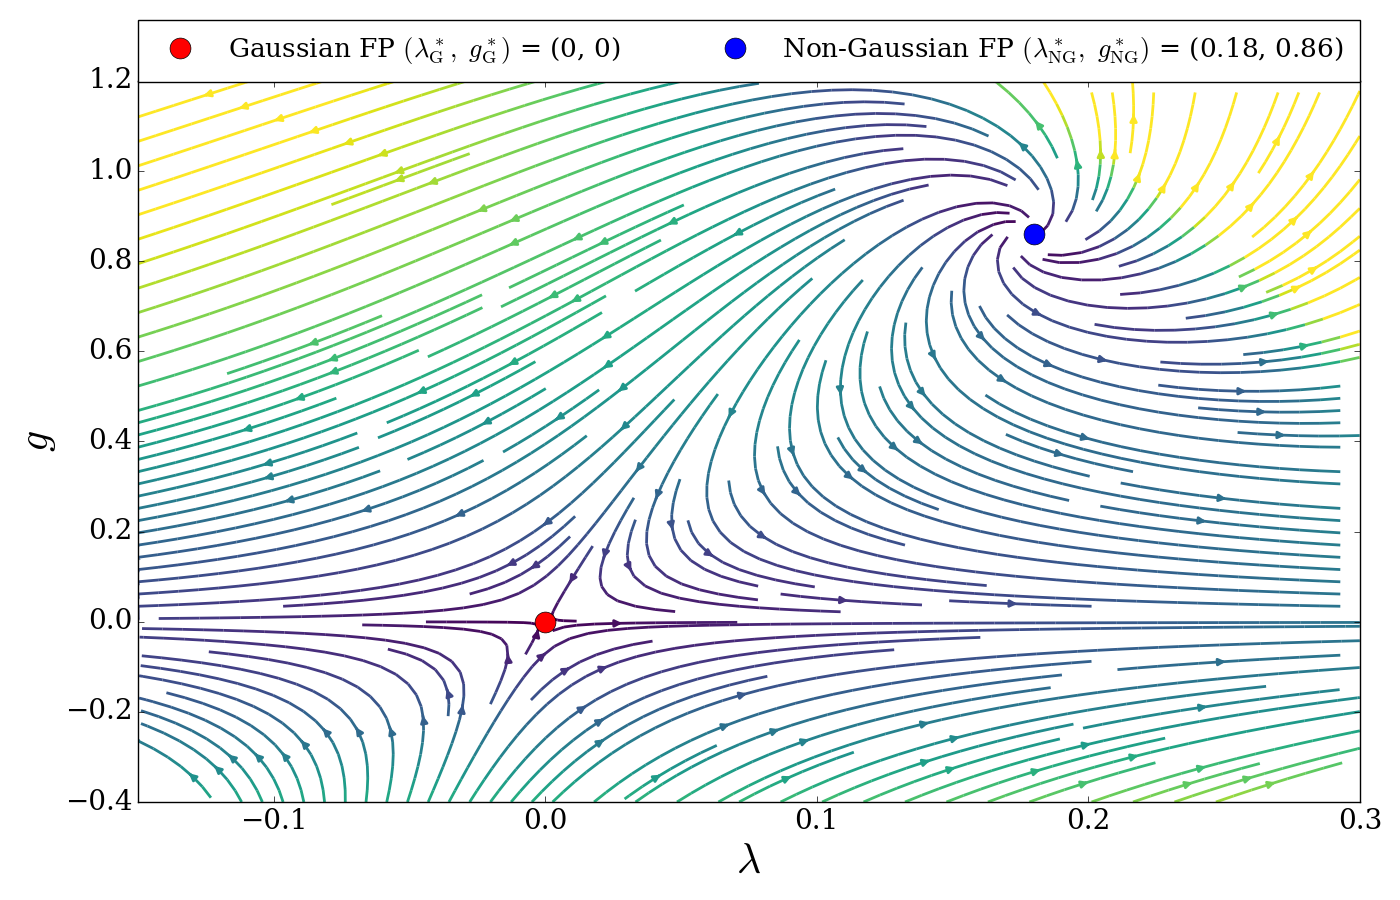
\includegraphics[width=0.8\textwidth]{figs/Plots/EH_NoMatter}
	\caption[Flow diagram for the Einstein-Hilbert truncation in $h^{\mathrm{TT}}$ approximation]{Flow diagram  for the Einstein-Hilbert truncation in $h^{\mathrm{TT}}$ approximation as computed in this work. The flow points towards the infrared. The postulated UV-attractive Non-Gaussian fixed point (blue dot) is clearly visible. }
	\label{fig:flow_diag}
\hrulefill	
\end{figure}
The corresponding flow diagram is depicted in figure  (\ref{fig:flow_diag}). The \enquote{swirl} around the NGFP is explained by the fact, that $\mathfrak{Im}\ \theta_{1,2} \neq 0$. The visualization and the plotting of the diagram was done in \verb|Python|.\\
Based on the results obtained in the scope of this calculation, we can confirm the existence of a UV-attractive Non-Gaussian Fixed point for this truncated pure-gravity system, providing a good starting point for further analysis. As a first extension of this truncation, we want to go beyond the $h^{\mathrm{TT}}$ approximation by taking the contributions for the other modes into account. Then, we will investigate the impact of minimally coupled matter fields on the system. All these calculations will be explained in full detail in the next chapter. 